\documentclass{beamer}

\usepackage[utf8]{inputenc}
\usepackage[spanish]{babel}
\usepackage[T1]{fontenc}
\usepackage{graphicx}
\usepackage{tikz}

\renewcommand\shorthandsspanish{}
\noextrasspanish

\title{Python}
\author{
Guillem Borrell i Nogueras\\
\texttt{guillemborrell@gmail.com}
}

\begin{document}

\begin{frame}
\begin{center}
 
\includegraphics[width=9cm]{files/python-logo-generic.pdf}\\
 % python-logo-generic.pdf: 389x115 pixel, 72dpi, 13.72x4.06 cm, bb=0 0 389 115
\begin{large}
\textbf{Python en Supercomputación}
\end{large}\\
Charla introductoria\\

Guillem Borrell i Nogueras\\

ETSIA, Octubre 2007
\end{center}

\end{frame}


\begin{frame}
 \frametitle{Preguntas...}
 \begin{itemize}
 \item ¿Por qué se llama Python?
 \item ¿Quién usa Python?
 \item ¿Para qué sirve Python?
 \begin{itemize}
  \item Principales características de Python
 \end{itemize}
 \item ¿Por qué Python se está volviendo tan popular?
 \item ¿Por qué Python y no otro lenguaje?
 \item ¿Qué puede ofrecer Python al HPC?
 \begin{itemize}
   \item Inconvenientes de Python
 \end{itemize}
  \item Ejemplos
 \end{itemize}

\end{frame}

\begin{frame}
 \frametitle{¿Por qué se llama Python?}
 Python debe su nombre a...
\end{frame}

\begin{frame}
 \begin{center}
 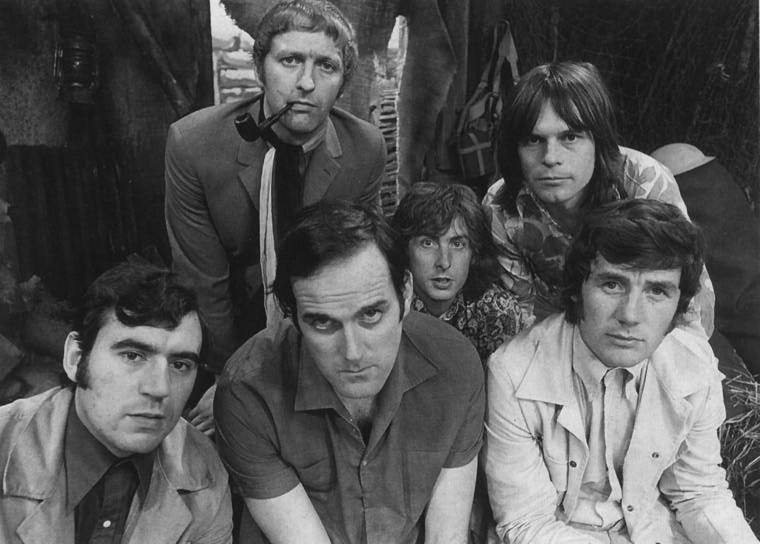
\includegraphics[width=9cm]{files/python.jpg}\\
 % python.jpg: 760x544 pixel, 72dpi, 26.81x19.19 cm, bb=0 0 760 544
Monty Python
\end{center}

\end{frame}

\begin{frame}
 \frametitle{¿Quién usa Python?}

\begin{center}
 
\includegraphics[width=3cm]{files/google.jpg}
 
\includegraphics[width=3cm]{files/Industrial_Light_and_Magic.jpg}
 
\includegraphics[width=3cm]{files/NASA_Logo.jpg}
 
\includegraphics[width=3cm]{files/honeywell_logo.jpg}
\end{center}
\end{frame}

\begin{frame}
 \frametitle{¿Para qué sirve Python?}
 \begin{center}
 Prácticamente para cualquier cosa que se nos pueda ocurrir
 \end{center}

\end{frame}

\begin{frame}
 \frametitle{Desde páginas web...}
\begin{center}
 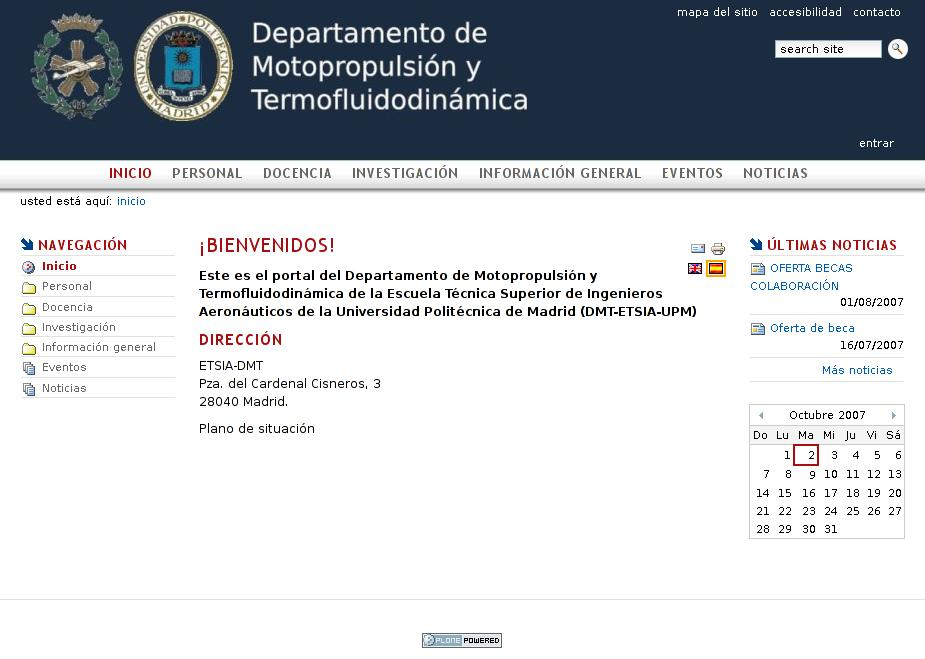
\includegraphics[width=9cm]{files/snapshot1.jpg}\\
 % snapshot1.jpg: 925x659 pixel, 762dpi, 3.08x2.20 cm, bb=0 0 87 62
Plone, Zope
\end{center}

\end{frame}

\begin{frame}
 \frametitle{...A utilidades para bioinformática}
\begin{center}
 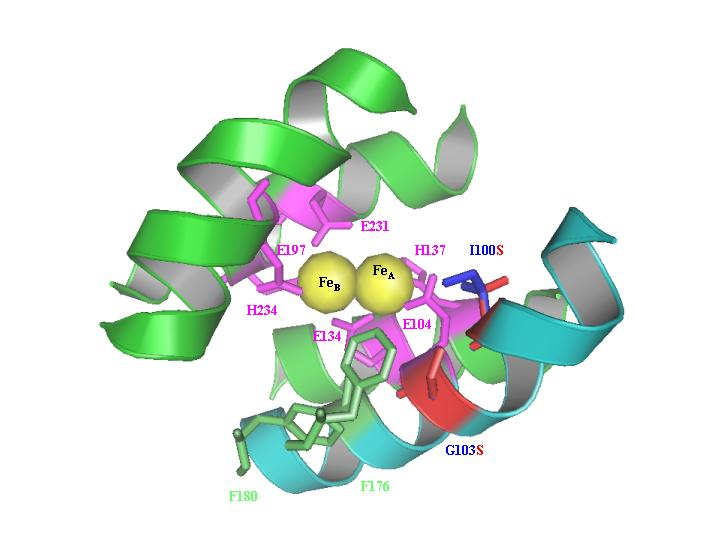
\includegraphics[width=8cm]{files/pymol.jpg}\\
 % pymol.jpg: 720x540 pixel, 72dpi, 25.40x19.05 cm, bb=0 0 720 540
Pymol
\end{center}

\end{frame}

\begin{frame}
 \frametitle{Principales características de Python}

\begin{itemize}
 \item Software Libre (Licencia estilo BSD)
 \item Interpretado
 \item Interactivo
 \item Multiparadigma
 \begin{itemize}
  \item Procedimental
  \item Modular
  \item Orientado a Objetos
 \end{itemize}
 \item Multiplataforma
 \item Especificación especialmente corta (IronPython, Jython, PyPy, Stackless)
 \item \emph{Incluye las pilas}
 \item ...
\end{itemize}

\end{frame}

\begin{frame}
 \frametitle{¿Por qué Python se está volviendo tan popular}
\begin{itemize}
 \item Fácil de aprender
 \item Fácil de ampliar
 \item Consistente por diseño
 \item Impone un buen estilo de programación
 \item Soporta todas las prácticas propuestas por XP, Agile.
\end{itemize}
\begin{center}
 Porque es divertido
\end{center}

\end{frame}

\begin{frame}
 \frametitle{¿Por qué Python y no otro lenguaje?}
\begin{itemize}
 \item Fácilmente extensible
 \begin{itemize}
 \item CPython, escrito en ANSI C
\end{itemize}
 \item Duck Typing (VS. Java y C++)
 \item Software Libre
 \item Excelente documentación
\end{itemize}

\end{frame}


\begin{frame}
\begin{center}
\begin{LARGE}
¿Qué pinta tiene código escrito en Python?
\end{LARGE} 
\end{center}
\end{frame}

\begin{frame}[containsverbatim]
 \frametitle{Todo es un objeto}
\begin{verbatim}
guillem@aiguaviva ~ $ python
Python 2.4.4 (#1, Sep 25 2007, 21:44:53)
[GCC 4.1.2 (Gentoo 4.1.2)] on linux2
Type "help", "copyright", "credits" or "license" ...
>>> import cmath
>>> i=cmath.sqrt(-1) #Los namespaces son objetos
>>> i.conjugate() #Los números son objetos
-1j
>>> i.imag
1.0
>>> i.real
0.0
>>> i+=3 
>>> i
(3+1j)
\end{verbatim}
\end{frame}

\begin{frame}[containsverbatim]
 \frametitle{Definir funciones es muy fácil}
\begin{verbatim}
>>> def sumauno(numero):
...     return numero+1
...
>>> sumauno(i)
(4+1j)
\end{verbatim}
\begin{itemize}
 \item No hay llaves ni ends, los niveles se definen por el sangrado.
\end{itemize}
\end{frame}

\begin{frame}[containsverbatim]
 \frametitle{Documentación a la Matlab}
\begin{verbatim}
>>> def docfunc():
...     """Esta es una función documentada, a diferencia
...     de Matlab la documentación de las funciones de
...     Python es extraíble y formateable"""
...     pass
...
>>> help(docfunc)
Help on function docfunc in module __main__:

docfunc()
    Esta es una función documentada, a diferencia de
    Matlab la documentación de las funciones de Python
    es extraíble y formateable
\end{verbatim}
\end{frame}


\begin{frame}[containsverbatim]
\frametitle{Una clase llamada pato}
\begin{verbatim}
 >>> class pato:
...     cantidad = 1
...     def haz_cua(self):
...           print "cua!"
...
...     def reproducete(self):
...           cantidad += 1
...
>>> estoesunpato=pato() #instancia de pato
>>> estoesunpato.cantidad
1
>>> estoesunpato.haz_cua()
cua!
\end{verbatim} 
\end{frame}

\begin{frame}[containsverbatim]
 \frametitle{Duck Typing}
Si algo anda como un pato y hace cua como un pato para mi va a ser un pato.
\begin{verbatim}
>>> estoesunpato=pato() #instancia de pato
>>> cuaqueador(estoesunpato)
cua!
>>> class guillem:
...     def haz_cua(self):
...             print "cua!"
...
>>> falsopato=guillem() #ese soy yo
>>> cuaqueador(falsopato)
cua!
>>> isinstance(falsopato,pato)
False
\end{verbatim}
Para la función cuaqueador yo soy tan pato como un pato.
\end{frame}

\begin{frame}
 \begin{center}
 \begin{Huge}
  Y mucho más...
 \end{Huge}
\end{center}
\end{frame}


\begin{frame}
 \frametitle{¿Qué puede ofrecer Python al HPC?}
Python es lento, $\sim 10 \times$C; Python pretende completar C y Fortran, no sustituirlos.
\vspace{1cm}
\begin{center}
Sirve para...\\
\vspace{1cm}
 \begin{Huge}
  Manejar la Complejidad
 \end{Huge} 
\end{center}
Wrappers, Interfaces, Prototipado, Scripting...
\end{frame}

\begin{frame}
 \frametitle{Inconvenientes de Python (para HPC)}
\begin{itemize}
 \item Diseño \emph{Single Thread} \textcolor{red}{(GIL)!}
 \item Implementación limpia vs. optimizada
 \item Librería estándar escrita en python (20\%-30\%  C)
 \item Versatilidad vs. potencia.
 \item \textcolor{red}{No hay una implementación propia de Arrays y Buffers}
 \item Es interpretado (¿?)
\end{itemize}
\end{frame}

\begin{frame}
 \frametitle{Soluciones a los inconvenientes}
\begin{itemize}
 \item Inlining (Weave)
 \item Extending (ctypes)
 \item Paralelo (PyMPI, ctypes, ParallelPython)
 \item \textcolor{red}{PyPy}
 \item Stackless
 \item Numpy, Scipy...
\end{itemize}
\end{frame}

\begin{frame}
 \frametitle{Numpy}
Es una extensión de Python que soporta arrays n-dimensionales\\
\vspace{2cm}
\begin{large}
Es una maravilla, verdad verdadera. Lástima que no se pueda demostrar en una transparencia 
\end{large}
\end{frame}

\begin{frame}[containsverbatim]
 \frametitle{Una pequeña introducción}
\begin{verbatim}
>>> import numpy as N
>>> x=N.array([[1,2,3,2],[2,3,4,3],
               [2,3,4,3],[3,2,3,4]],'d')
>>> N.fft.rfft2(x)
array([[ 44.+0.j,  -6.+2.j,   0.+0.j],
       [ -4.+0.j,  -2.+2.j,   0.+0.j],
       [ -4.+0.j,  -2.-2.j,   0.+0.j],
       [ -4.+0.j,   2.-2.j,   0.+0.j]])
>>> x.transpose()
array([[ 1.,  2.,  2.,  3.],
       [ 2.,  3.,  3.,  2.],
       [ 3.,  4.,  4.,  3.],
       [ 2.,  3.,  3.,  4.]])
\end{verbatim}
\end{frame}

\begin{frame}
 \frametitle{¿Cuál es la idea entonces?}
Introducir Python en HPC $\Leftrightarrow$ Crear una aplicación multilenguaje.

\begin{center}
 \begin{tikzpicture}
  \draw[->,thick] (0,0) -- (4.5,0) node[right] {complejidad};
  \draw[->,thick] (0,0) -- (0,4.5) node[above] {rendimiento};
  \fill[green,semitransparent] (0,0) rectangle (2.25,2.25);
  \fill[magenta,semitransparent] (2,0) rectangle (4,2);
  \fill[cyan,semitransparent] (0,2) rectangle (2,4);
  \fill[yellow,semitransparent] (1.75,1.75) rectangle (4,4);
  \draw (5,1.25) node[draw,right] (matlab) {Matlab};
  \draw (5,2.25) node[draw,right] (python) {Python};
  \draw (5,3.25) node[draw,right] (fc) {Fortran, C};
  \draw (5,4.25) node[draw,right] (pfc) {Python + Fortran,C};
  \draw[->] (pfc) -- (3,3);
  \draw[->] (matlab) -- (1,1);
  \draw[->] (python) -- (3,1);
  \draw[->] (fc) -- (1,3);
 \end{tikzpicture}

\end{center}

\end{frame}

\begin{frame}
 \frametitle{¿Qué se gana añadiendo Python a C, Fortran?}
\begin{itemize}
 \item Namespaces
 \item Abstracción (Modularidad, OO)
 \item Añadir interactividad
 \item Autodocumentación
 \item Crear cajas negras
 \begin{itemize}
  \item Si no tengo que saberlo no me lo cuentes
  \item Si no tengo que verlo no me lo enseñes
  \item Si algo funciona bien, recíclalo
 \end{itemize}
\end{itemize}
\end{frame}

\begin{frame}
 \frametitle{¿Cómo se añade Python a C y Fortran?}
\begin{center}
 Haciendo Wrappers\\
\vspace{1cm}
\begin{tikzpicture}
 \draw (0,0) node[draw] (cf) {C, Fortran};
 \draw (2,0) node (wrapper) {Wrapper};
 \draw (4,0) node[draw] (python) {Python};
 \draw[->] (cf) -- (wrapper);
 \draw[->] (wrapper) -- (python);
\end{tikzpicture}
\\
\end{center}
Objetivo: crear un Matlab $\copyright$ muy personalizado.
\begin{itemize}
 \item Ventajas
 \begin{itemize}
 \item Añaden interactividad, potencia, versatilidad...
 \item No hay que repetirlos
 \end{itemize}
 \item Inconvenientes
 \begin{itemize}
 \item Más decisiones de diseño
 \item Requieren más esfuerzo
 \end{itemize}
 \end{itemize}
\end{frame}

\begin{frame}
 \begin{center}
  \begin{Huge}
   ¿Por qué Python?
  \end{Huge}
\end{center}
\end{frame}

\begin{frame}
 Porque en muchos casos:
\begin{itemize}
 \item Los wrappers ya estarán hechos (lapack, blas, fftpack, mpi)
 \item Hacerlos requerirá un esfuerzo mínimo
\end{itemize}
Gracias a:
\begin{itemize}
 \item \textbf{ctypes}
 \item \textbf{f2py} (Fortran)
 \item SWIG (C, C++)
 \item weave
 \item ...
\end{itemize}
\end{frame}

\begin{frame}
\begin{center}
 \begin{Huge}
  Continuará...
 \end{Huge}
\end{center}
\end{frame}

\begin{frame}
 \frametitle{Charla técnica}
\begin{itemize}
 \item Python Vs. Matlab.
 \item Más sobre los wrappers.
 \item Arrays en C, Fortran y Python.
 \item GIL.
 \item Uso de F2Py.
 \item ctypes.
 \item Python en paralelo.
\end{itemize}

\end{frame}



\end{document}